\section{Auswertung}
\label{sec:Auswertung}

\subsection{Bestimmung von $\frac{h}{e}$ und der Austrittsarbeit}

Es werden die zwischen Photokathode und Anode angelegte Gegenspannung $U$, sowie der 
Photostrom $I$ für alle erkennbaren Spektrallinien durchgemessen und $\sqrt{I}$ berechnet. 
Diese Messdaten finden sich in den Tabellen \ref{tab:gelb} bis \ref{tab:blau}. 

\begin{table}
    \centering
    \caption{Gelb}
    \label{tab:gelb}
    \sisetup{table-format=2.1}
    \begin{tabular}{c c c}
    \toprule
    $ U \;/\; \si{\volt} $ & $I \;/\; \si{\nano\ampere}$ &
    $ \sqrt{\frac{I}{\si{\nano\ampere}}}$\\
    \midrule 
      -0.670 & 0.000 & 0.000\\
      -0.500 & 0.002 & 0.045\\
      -0.250 & 0.014 & 0.118\\
       0.000 & 0.029 & 0.170\\
       0.250 & 0.042 & 0.205\\
       0.500 & 0.055 & 0.235\\
       0.750 & 0.066 & 0.257\\
       1.000 & 0.077 & 0.277\\
       1.250 & 0.086 & 0.293\\
       1.500 & 0.096 & 0.310\\        
    \bottomrule
    \end{tabular}
\end{table}

\begin{table}
    \centering
    \caption{Grün}
    \label{tab:gruen}
    \sisetup{table-format=2.1}
    \begin{tabular}{c c c}
    \toprule
    $ U \;/\; \si{\volt} $ & $I \;/\; \si{\nano\ampere}$ &
    $ \sqrt{\frac{I}{\si{\nano\ampere}}}$\\
    \midrule 
       -0.650 & 0.000 & 0.000\\   
       -0.500 & 0.002 & 0.045\\  
       -0.250 & 0.018 & 0.134\\  
        0.000 & 0.034 & 0.184\\ 
        0.250 & 0.048 & 0.219\\  
        0.500 & 0.062 & 0.249\\
        0.750 & 0.073 & 0.270\\  
        1.000 & 0.085 & 0.292\\  
        1.500 & 0.120 & 0.346\\ 
        2.000 & 0.140 & 0.374\\ 
        3.000 & 0.190 & 0.436\\       
    \bottomrule
    \end{tabular}
\end{table}

\begin{table}
    \centering
    \caption{Violett}
    \label{tab:viol}
    \sisetup{table-format=2.1}
    \begin{tabular}{c c c}
    \toprule
    $ U \;/\; \si{\volt} $ & $I \;/\; \si{\nano\ampere}$ &
    $ \sqrt{\frac{I}{\si{\nano\ampere}}}$\\
    \midrule 
      -1.130 & 0.0000 & 0.000\\
      -1.000 & 0.0020 & 0.045\\
      -0.750 & 0.0130 & 0.114\\
      -0.500 & 0.0295 & 0.172\\
      -0.250 & 0.0520 & 0.228\\
       0.000 & 0.0730 & 0.270\\
       0.250 & 0.1100 & 0.332\\
       0.500 & 0.1300 & 0.361\\
       0.750 & 0.1500 & 0.387\\
       1.000 & 0.1700 & 0.412\\     
    \bottomrule
    \end{tabular}
\end{table}

\begin{table}
    \centering
    \caption{Blau}
    \label{tab:blau}
    \sisetup{table-format=2.1}
    \begin{tabular}{c c c}
    \toprule
    $ U \;/\; \si{\volt} $ & $I \;/\; \si{\nano\ampere}$ &
    $ \sqrt{\frac{I}{\si{\nano\ampere}}}$\\
    \midrule 
      -1.270 & 0.000 & 0.000\\
      -1.000 & 0.003 & 0.055\\
      -0.750 & 0.008 & 0.089\\
      -0.500 & 0.010 & 0.100\\
      -0.250 & 0.025 & 0.158\\
       0.000 & 0.035 & 0.187\\
       0.250 & 0.044 & 0.210\\
       0.500 & 0.052 & 0.228\\
       0.750 & 0.062 & 0.249\\
       1.000 & 0.069 & 0.263\\ 
    \bottomrule
    \end{tabular}
\end{table}

%\begin{table}
%    \centering
%    \caption{Orange}
%    \label{tab:orange}
%    \sisetup{table-format=2.1}
%    \begin{tabular}{c c c}
%    \toprule
%    $ U \;/\; \si{\volt} $ & $I \;/\; \si{\nano\ampere}$ &
%    $ \sqrt{\frac{I}{\si{\nano\ampere}}}$\\
%    \midrule 
%      -1.000 & 0.000 & 0.000\\
%      -0.500 & 0.002 & 0.045\\
%      -0.250 & 0.009 & 0.095\\
%       0.250 & 0.031 & 0.145\\
%       0.000 & 0.021 & 0.176\\
%       0.500 & 0.042 & 0.205\\
%       0.750 & 0.052 & 0.228\\
%       1.000 & 0.062 & 0.249\\
%    \bottomrule
%    \end{tabular}
%\end{table}

Nun wird mittels Python und Matplotlib für jede Spektrallinie eine lineare Ausgleichsrechung durchgeführt, indem 
$\sqrt{I}$ gegen die Gegenspannung $U$ aufgetragen wird. Die Plots sind in Grafik \ref{fig:plot1} zu sehen.

\begin{figure}
  \centering
  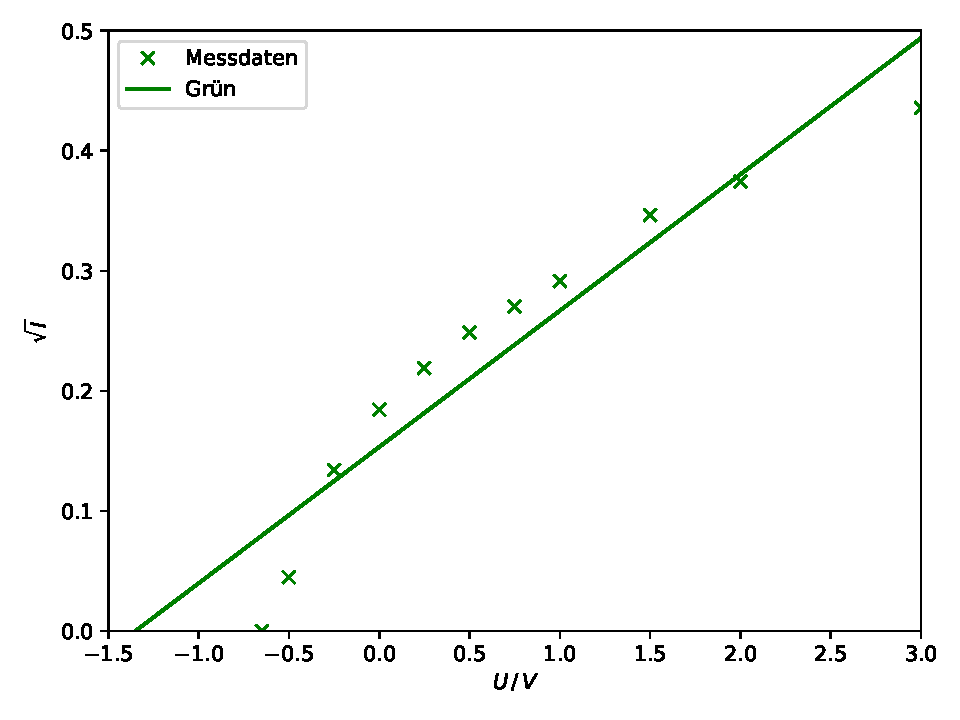
\includegraphics{content/plot1.pdf}
  \caption{Messdaten von verschiedenen Spektrallinien und Regressionen.}
  \label{fig:plot1}
\end{figure}

Die mit den Ausgleichsgeraden der Form 

\begin{equation*}
\sqrt{\frac{I}{nA}} = a\cdot U + b 
\end{equation*}

erhaltenen Regressionsparameter sind für die zugehörigen Wellenlänge in $\lambda$ in Tabelle \ref{tab:para} aufgeführt. 

\begin{table}
    \centering
    \caption{Parameter der linearen Fits.}
    \label{tab:para}
    \sisetup{table-format=2.1}
    \begin{tabular}{c c c}
    \toprule
    $ \lambda \;/\; \si{\nano\meter} $ & $a \;/\; \si{\volt\second}$ &
    $ b \;/\; \si{\volt}$\\
    \midrule 
      546.00 & $\num{0.114+-0.014}$ & $\num{0.153+-0.018}$\\ %grün
      435.80 & $\num{0.195+-0.013}$ & $\num{0.251+-0.009}$\\ %violett
      576.96 & $\num{0.138+-0.016}$ & $\num{0.138+-0.013}$\\ %gelb
      404.70 & $\num{0.115+-0.008}$ & $\num{0.169+-0.006}$\\ %blau
    \bottomrule
    \end{tabular}
\end{table}

Aus den Schnittpunkten mit der Spannungsachse ergeben sich somit die Grenzspannungen, 
diese sind in Tabelle \ref{tab:gegen} eingetragen. 

\begin{table}
    \centering
    \caption{Schnittpunkte mit der Spannungsachse}
    \label{tab:gegen}
    \sisetup{table-format=2.1}
    \begin{tabular}{c c}
    \toprule
    $ \lambda \;/\; \si{\nano\meter} $ & $U_\text{g} \;/\; \si{\volt}$\\
    \midrule 
      546.00 & $\num{-1.35}$\\ %grün
      435.80 & $\num{-1.30}$\\ %violett
      576.96 & $\num{-1.00}$\\ %gelb
      404.70 & $\num{-1.45}$\\ %blau
    \bottomrule
    \end{tabular}
\end{table}

Mit den erhaltenen Gegenspannungen und den Lichtfrequenzen wird eine weitere Ausgleichsrechnung 
durchgeführt. Dazu werden die negativen Vorzeichen weggelassen, da sonst mit $E = U\cdot e$ eine 
negative Energie der Elektronen folgen würde. Das Ergebnis hierzu ist in Abbildung \ref{fig:plot2} zu 
begutachten. 

\begin{figure}
  \centering
  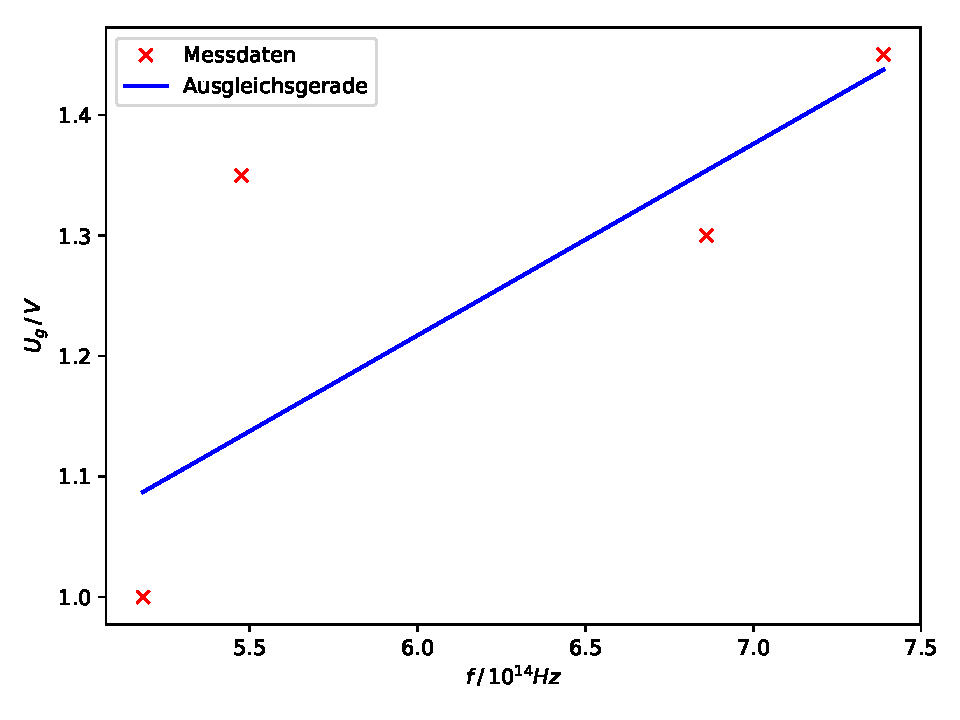
\includegraphics{content/plot2.pdf}
  \caption{Die zuvor berechneten Spannungswerte gegen die jeweilige Frequenz.}
  \label{fig:plot2}
\end{figure}

Mit der Ausgleichsgeraden

\begin{equation*}
U_\text{g} = a\cdot f + b
\end{equation*}

werden die Werte

\begin{align*}
a &= \SI{0.159+-0.123e-14}{\volt\second},\\
b &= \SI{0.264+-0.750}{\volt}
\end{align*}

erhalten.
Die Steigung $a$ ist nun genau $\frac{h}{e}$, also $h$ in $\si{\eV}$ angegeben, da $U = \frac{E}{e}$. Der 
Achsenabschnitt $b$ entspricht aufgrund der gleichen Beziehung genau der Austrittsarbeit in $\si{\eV}$.
Somit ergeben sich die gesuchten Größen: 

\begin{align*}
h &= \SI{1.59e-15}{\eV\second},\\
E_\text{A} &= \SI{0.264}{\eV}.
\end{align*}

\subsection{Betrachtung des Photostroms in Abhängigkeit der Spannung}

Im zweiten Versuchsteil wird der Photostrom $I$ in Abhängigkeit der angelegten Spannung $U$
betrachtet, wobei die Spannung im Bereich vom $\SI{-10}{\volt}$ bis $\SI{19}{\volt}$ variiert 
wird. Die gemessenen Wertepaare bei der konstanten Wellenlänge $\lambda = \SI{578}{\nano\meter}$
sind in Tabelle \ref{tab:stsp} aufgeführt. 

\begin{table}
    \centering
    \caption{Strom-Spannungs-Messwerte}
    \label{tab:stsp}
    \sisetup{table-format=2.1}
    \begin{tabular}{c c}
    \toprule
    $ U \;/\; \si{\volt} $ & $I \;/\; \si{\nano\ampere}$\\
    \midrule 
      -10.000 & 0.0035\\
       -8.000 & 0.0030\\
       -3.500 & 0.0020\\
       -2.500 & 0.0020\\
       -1.750 & 0.0020\\
       -1.500 & 0.0020\\
       -1.250 & 0.0020\\
       -1.000 & 0.0015\\
       -0.750 & 0.0010\\
       -0.670 & 0.0000\\ 
       -0.500 & 0.0020\\
       -0.250 & 0.0140\\
        0.000 & 0.0290\\
        0.250 & 0.0420\\
        0.500 & 0.0550\\
        0.750 & 0.0660\\
        1.000 & 0.0770\\
        1.250 & 0.086\\
        1.500 & 0.096\\
        1.750 & 0.119\\
        2.000 & 0.120\\
        2.500 & 0.150\\
        3.000 & 0.170\\
        3.500 & 0.190\\
        4.000 & 0.205\\
        4.500 & 0.220\\
        5.000 & 0.225\\
        6.000 & 0.245\\
        7.000 & 0.260\\
        8.000 & 0.280\\
        9.000 & 0.295\\
       10.000 & 0.300\\
       11.000 & 0.315\\
       12.000 & 0.325\\
       13.000 & 0.340\\
       14.000 & 0.345\\
       15.000 & 0.350\\
       16.000 & 0.360\\
       17.000 & 0.370\\
       18.000 & 0.380\\
       19.000 & 0.380\\
       \bottomrule
    \end{tabular}
\end{table}

Graphisch aufgetragen ergibt sich in Abbildung \ref{fig:plot3}. 

\begin{figure}
  \centering
  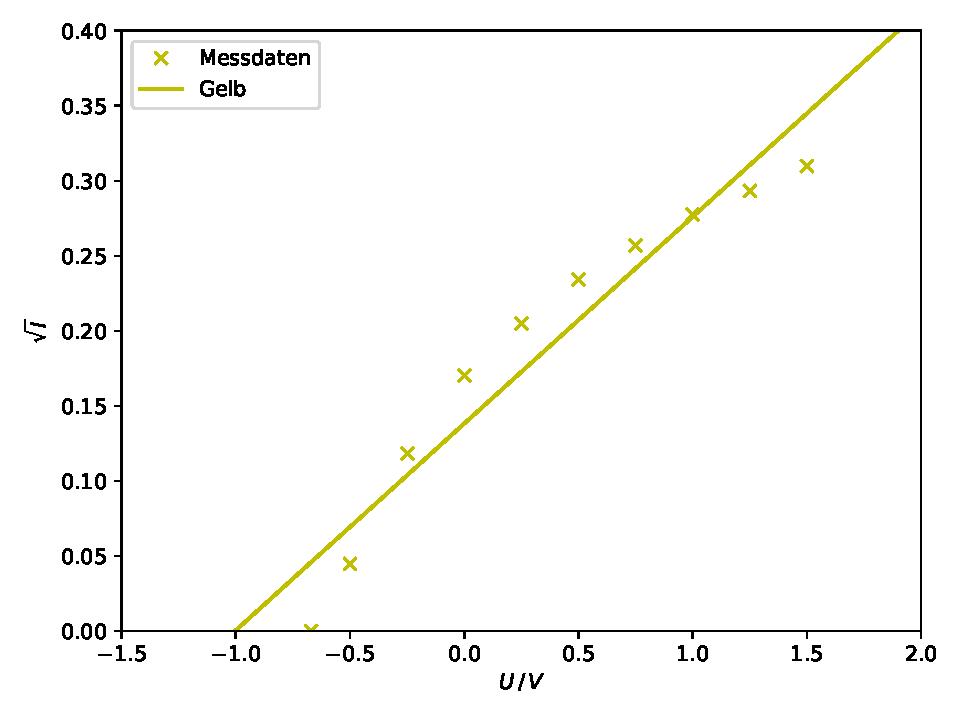
\includegraphics{content/plot3.pdf}
  \caption{Aufgenommene Kennlinie bei $\lambda=\SI{578}{\nano\meter}$.}
  \label{fig:plot3}
\end{figure}

Es ist ersichtlich, dass die aufgenommene Kurve bei positiven, beschleunigenden Spannungen 
gegen einen Sättigungswert geht. D.h. die Stromstärke nähert sich asymptotisch einer 
maximalen Stromstärke. Die Existenz eines solchen Sättigungswertes lässt sich einfach 
durch die konstante Intensität erklären. Da diese direkt proportional zur Anzahl der 
austretenden Elektronen ist, muss somit auch der Stromfluss durch eine Konstante 
beschränkt sein. Das Ohmsche Gesetz kann daher nicht angewandt werden. Die Tatsache, 
das dieser Sättigungswert nur asymptotisch erreicht wird, liegt darin begründet, dass 
die Elektronen mit verschiedenen Energiewerten aus der Photokathode austreten. Dadurch 
kann der Sättigungswert nicht ab einer Grenzspannung plötzlich auftreten, sondern sich 
nur asymptotisch dem Sättigungswert nähern. Außerdem deckt die Ringanode nur einen kleinen
Raumbereich ab, sodass ohnehin nur ein Bruchteil der Photoelektronen aufgefangen werden kann. 
Zum vollständigen Erreichen des maximalen Stromflusses bei einer endlichen Spannung müsste 
die Anode alle ausgelösten Elektronen auffangen. \\
Außerdem wird erkannt, dass der Strom im Bereich der Gegenspannung nicht unstetig auf 0 
springt, sondern für $U\rightarrow U_\text{g}$ allmählich auf 0 absinkt. Dies liegt ebenfalls 
in der Energieverteilung der Elektronen begründet. Da diese in der Photokathode einer 
Fermi-Dirac-Statistik genügen, haben die Elektronen vor dem Austritt verschiedene Energiewerte. 
Auch nach dem Austritt liegt diese ungleiche Verteilung vor, da prinzipiell jedes Elektron 
den gleichen Energiebetrag von $E=h\cdot f$ zugeführt bekommt.\\
Weiterhin wird erkannt, dass im Bereich Gegenspannung $U < U_\text{g}$ ein geringfügiger, 
entgegengerichteter Stromfluss messbar ist, welcher bereits bei kleinen Spannungswerten 
einen Sättigungswert annimmt. Dieser Effekt lässt sich dadurch erklären, dass die 
Beschichtung der Photokathode bereits bei geringen Temperaturen anfängt zu verdampfen. 
Diese so erzeugten, freien Atome werden dann durch den auftretenden Photoeffekt ionisiert
und wandern aufgrund ihrer positiven Ladung zur Anode. Dort lösen sie Elektronen aus, um sich 
wieder zu neutralisieren. Anschließend können sie erneut ionisiert werden und so weiter. Das bei 
der Ionisierung frei werdende Elektron hingegen wandert zur Photokathode. So entsteht insgesamt 
ein Strom in entgegengesetzer Richtung. Man erkennt, dass dieser Effekt eindeutig von der 
Teilchendichte der freien Atome im Vakuum abhängt. Da diese aber nicht beliebig hoch werden kann und 
die Metallatome der Photokathode auch kondensieren, gibt es einen Sättigungswert des Stromes. Die 
Tatsache, dass dieser Effekt bereits bei energiearmen Licht (ca. $\SI{650}{\nano\meter})$ auftritt, 
beweist, dass die Anode eine sehr geringe Austrittsarbeit $E_\text{A} = \SI{1.9}{\eV}$ haben muss. 
Dies leitet sich daraus ab, dass ein Atom im freien Raum mit genau dieser Energie ionisiert werden 
kann und genau diesen Energiebetrag dazu verwendet, um ein Elektron aus der Anode herauszulösen. 